\title{Dataset Description}

\documentclass[12pt]{article}
\usepackage{graphicx}

\begin{document}
\maketitle

In PaCMan Shape Dataset, we have collected 400 objects consisting of 20 categories, each having 20 models. The categories consist of household objects: Mug, cup, fork, jug, plate, bowl, frying pan, tray, teapot, tea cup, cutting board, box, knife, vase, can, fork, spatula, scissors, bottle and shaker. The objects have realistic sizes, and their longest dimension range from 80 mm to 200 mm, depending on the category. One representative image out of every class is depicted in Fig. \ref{shapes}.

 \begin{figure}[!h]
  \caption{Representative shapes for every class in the dataset.}
  \centering
    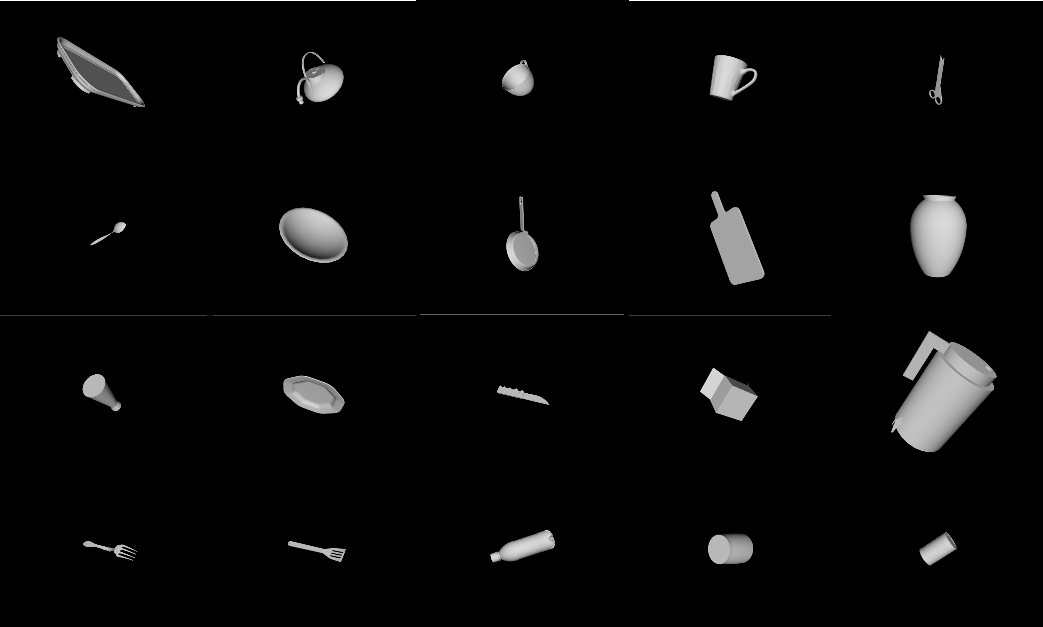
\includegraphics[width=\textwidth]{shapes.png}
\label{shapes}
\end{figure}

In order to render the objects from multiple viewpoints, we have used 32 uniformly sampled points on the view sphere. The azimuth and elevation of these samples are given below. Fig \ref{viewSphere} shows the triangulation of the view sphere, where every vertex corresponds to a camera position, with the viewing vector directed to the centre of the sphere. We have  rendered every object from each viewpoint using a simulated RGB camera and a depth camera, which has the characteristics of a Carmine 1.09 sensor.
 
 
\begin{itemize}
\item azimuth =(358, 62, 238, 272, 195, 167, 274, 50, 230, 242, 273, 92, 347, 314, 58, 134, 297, 336, 94, 308, 93, 254, 178, 156, 26, 184, 206, 4, 15, 128, 74, 117)
\item elevation = (58, -38, -2, -26, -18, 12, -68, 39, -39, 38, 12, 26, -12, -38, 2, 38, 42, 24, 68, -1, -12, 75, -58, -24, -17, 50, 17, 50, 18, 1, -75, -42)
\end{itemize}

\begin{figure}[!h]
  \caption{View sphere triangulation.}
  \centering
    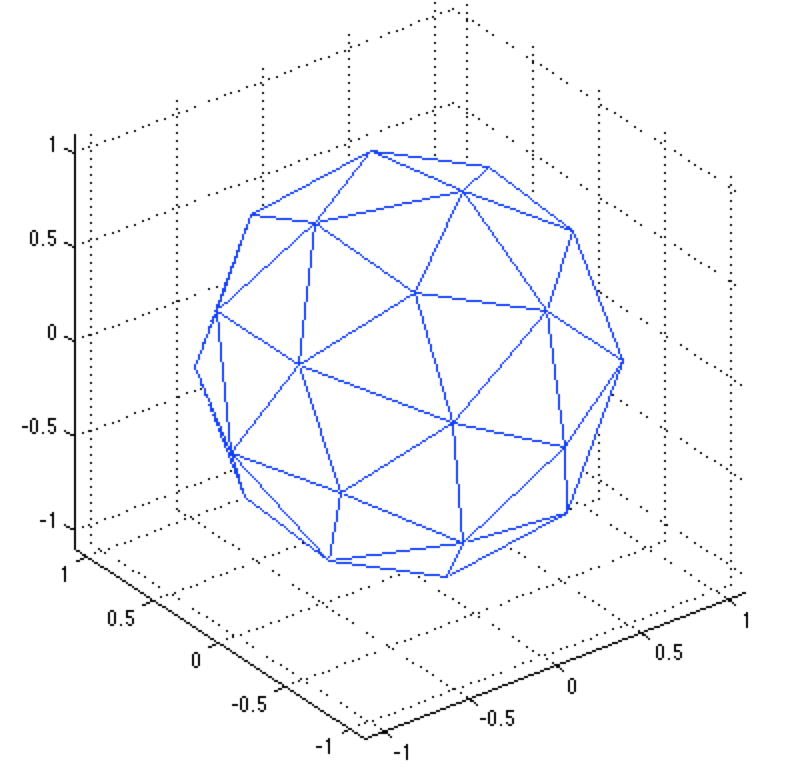
\includegraphics[width=0.6\textwidth]{viewSphere.png}
\label{viewSphere}
\end{figure}

The image acquisition process proceeds as follows:
\begin{enumerate}
\item Object is placed such that its centre of gravity is at the origin.
\item Camera is located on the y axis in various distances from the origin, namely, [0, 600mm, 0] or [0, 900mm, 0] or [0, 1200mm, 0].
\item Two light sources have been placed in the scene. The more powerful light source is located above the camera, while the weaker one is below the camera, with respect to the camera's up vector. This creates enough intensity differences to reveal intensity edges on the object. 
\item Camera is directed towards the origin. Camera has horizontal Field of View of 57.5 degrees.
\item Near range of the camera is 350mm, far range is 1400mm. That means that depth values in range from 350mm to 1400mm are encoded in 2 byte values. Larger values correspond to closer distances.
\end{enumerate}

Rendered images of the objects are placed in a hierarchical structure, and named in a specific way. For example, for a rendered image that has the name ``3\_P2\_IP3.png":
\begin{itemize}
\item 3 is the id of the object in the dataset (from 1 to 400)
\item P2 - that means that values a(2) and b(2) were used to rotate the object (we rotate the object, not the camera).
\item IP3 - id of the in-plane rotation. There are 8 ids in total, describing 8 rotation of the camera around y axis, with step size of 45 degrees. IP1 would correspond to zero orientation of the camera.
\end{itemize}

The category labels are stored in a 400x1 array that contains the label of every model in the dataset, distributed along with the images.

\bibliographystyle{abbrv}
\bibliography{main}

\end{document}
This is never printed
